%%========================Introducao================================%%
\section{Hiper Heurísticas}

%%========================Objetivo================================%%
\subsection{Hiper Heurísticas}
\frame{
	\frametitle{Hiper Heurísticas}
	

		\begin{itemize}
			\item   Apesar do sucesso de meta-heurísticas e outros métodos de busca ainda existem dificuldades de generalização destas estratégias. 
			\item  Esta dificuldade surge  da necessidade de selecionar
			os parâmetros e configurações mais adequados dos algoritmos para um problema ou instância.
			\item  Questão: \textbf{É possível
			automatizar o projeto e parametrização de métodos heurísticos para resolver problemas
			de busca computacional difíceis?}
			\item A ideia principal é desenvolver algoritmos que sejam
			mais genéricos do que as implementações de metodologias atuais.
		\end{itemize}
		
		

}


\frame{
	\frametitle{Hiper Heurísticas}
	

		\begin{itemize}
		\item Operam sobre o
		espaço de busca de heurísticas que operam sobre o espaço de busca  de um determinado problema.
		\item O objetivo
		principal é tentar encontrar ou construir a heurística mais adequada para cada
		situação.
		\item Geralmente \textit{frameworks} hiper-heurísticos possuem dois níveis: Alto e Baixo.
		\end{itemize}
}

\frame{
	\frametitle{Hiper Heurísticas}
		\begin{itemize}
	\item \textbf{Heurísticas de alto nível}: Geralmente consistem em dois componentes: \textbf{mecanismo
	de seleção}, que gerencia quais heurísticas de baixo nível devem ser aplicadas durante
	a busca; um \textbf{critério de aceitação}, que tem a responsabilidade de decidir se irá aceitar
	ou não uma solução gerada, a partir da aplicação de uma heurística de baixo nível.
	\item \textbf{Heurísticas de baixo nível}:  Um conjunto de heurísticas de baixo nível específicas.
	Estas heurísticas costumam diferir entre domínios de problemas. São exemplos: \textbf{operadores
	de cruzamento, mutação e buscas locais}. Em alguns casos, \textbf{meta-heurísticas} também,
	dependendo da modelagem do framework hiper-heurístico, podem assumir o papel de
	heurísticas de baixo nível.
			\end{itemize}

}




\subsection{Framework Geral Hiper Heurísticas}
\frame{
	\frametitle{\textit{Framework} Geral Hiper Heurísticas}

		\begin{figure}[!htb]
			\centering
			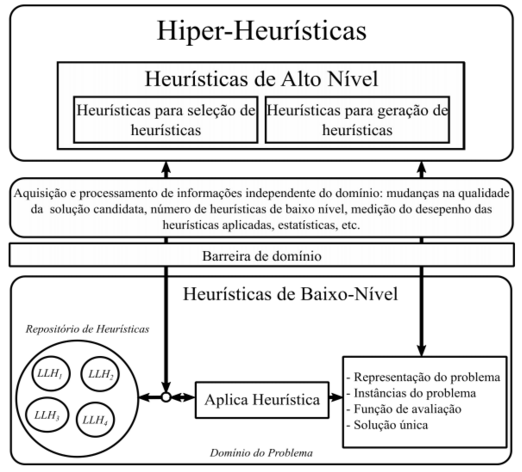
\includegraphics[scale=.6]{figuras/HiperHeuristicas.png}
			\caption{\textit{Framework} Geral Hiper-Heurístico. Adaptado de \cite{sabar2015automatic}}
			\label{img:hiperheuristico}
		\end{figure}

}

\subsection{Classificação Hiper Heurísticas}
\frame{
	\frametitle{Classificação Hiper Heurísticas}
	

		\begin{figure}[!htb]
			\centering
			\includegraphics[scale=.5]{figuras/ClassificacaoHiperHeuristica.png}
			\caption{Classificação Hiper Heurísticas}
			\label{fig:classificacaoHH}
		\end{figure}

}


\subsection{Hiper Heurísticas de Seleção}
\frame{
	\frametitle{Hiper Heurísticas de Seleção}
	

		\begin{itemize}
			\item \textbf{Random} (R):  Seleciona aleatoriamente as heurísticas a serem aplicadas.
			\item \textbf{Choice Function} (CF):  Função que leva em consideração o desempenho das heurísticas assim como quanto tempo se passou desde a última execução de uma heurística \cite{burke2013hyper}.
			\item \textbf{Greedy} (GR): Realiza as escolhas de maneira gulosa levando em consideração o desempenho das heurísticas \cite{burke2013hyper}.
			\item \textbf{Tabu Search Based} (TS): Utiliza uma lista tabu para evitar determinadas heurísticas que não apresentaram bom desempenho \cite{burke2013hyper}.
			\item \textbf{Multi-Armed Bandit} (MAB): Utiliza uma função baseada em dois componentes: um mede a qualidade de uma determinada heurística e está relacionado à intensificação e outro utiliza um intervalo de confiança baseado no número de vezes que a heurística foi aplicada \cite{burke2013hyper}.
		\end{itemize}

}


\subsection{Critérios de Aceitação}
\frame{
	\frametitle{Critérios de Aceitação}

			\begin{itemize}
				\item \textbf{All Moves} (AM): Aceita qualquer aplicação de heurísticas mesmo que seja sem melhora na solução \cite{burke2013hyper}.
				\item \textbf{Improvemnt Only} (IO): Aceita apenas aplicações de heurística que melhoraram uma solução \cite{burke2013hyper}.
				\item \textbf{Monte Carlo} (MC): Aceita aplicações de heurísticas que melhoram uma solução e utiliza probabilidades para aceitar aplicações que não melhoram \cite{burke2013hyper}.
				\item \textbf{Great Deluge} (GD): Esta estratégia estende o algoritmo \textit{Great Deluge} para decidir quando aceitar soluções geradas pelas heurísticas \cite{burke2013hyper}.				
			\end{itemize}
}



\subsection{Hiper-heurísticas de Geração}
\frame{
	\frametitle{Hiper-heurísticas de Geração}

		\begin{itemize}
			\item Estas hiper-heurísticas geram novas heurísticas combinando componentes de heurísticas.
			\item Geralmente se utiliza algum tipo de programação genética (PG), como por exemplo: evolução gramatical (EG) ou programação gênica.
		\end{itemize}

}



\subsection{Programação Genética (PG)}
\frame{
	\frametitle{Programação Genética (PG)}
		\begin{itemize}
			\item É um ramo da síntese de programas que utiliza ideias oriundas
			da teoria da evolução natural para produzir programas.
			\item Uma população aleatória de programas de computador é gerada, e os
			operadores geneticamente inspirados (cruzamento e mutação) são repetidamente aplicados
			com objetivo de produzir novos programas de computador.
			
			\item Estes programas são avaliados
			utilizando uma função de fitness que determina quais destes programas são mais
			suscetíveis a sobreviver para gerações futuras.
			\item Os programas
			que compõem a população são representados utilizando estruturas de árvore.
			\item Outras estruturas podem ser evoluídas.
		\end{itemize}

}


\subsection{Evolução Gramatical (EG)}
\frame{
	\frametitle{Evolução Gramatical (EG)}
	

		
		\begin{itemize}
		\item Técnica relativamente nova de computação evolutiva, proposta por Ryan et al. \cite{ryan1998grammatical}, trata-se de um tipo de programação genética. 
		\item Objetivo é encontrar um programa executável ou trecho
		de um programa, que obtenha um bom valor de \textit{fitness} para o problema em questão.
		\item Utiliza vetores de inteiros para representar seus indivíduos e uma gramática BNF específica para traduzir os indivíduos em programas de computador.
		\item Uma gramática BNF possui um 
		conjunto de terminais (+, -, *, /)  e não terminais, que podem ser expandidos em um ou mais terminais e
		não terminais.
		\end{itemize}

}

\subsection{Gramática Exemplo}
\frame{
	\frametitle{Gramática Exemplo}
	

			\begin{figure}[!htb]
				\centering
				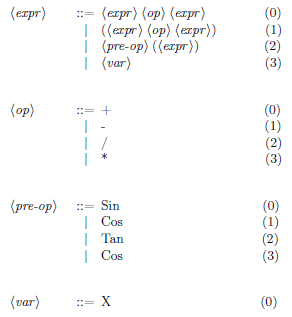
\includegraphics[scale=.8]{figuras/GramaticaExemplo.png}
				\caption{Gramática Exemplo}
				\label{fig:gramaticaExemplo}
			\end{figure}
	

}


\subsection{Hiper-heurísticas de Geração}
\frame{
	\frametitle{Operadores para evolução gramatical}
	

			 Além dos operadores tradicionais outros dois operadores \textit{Prune} e \textit{Duplicate} são peculiares à EG e serão descritos em seguida:
			 
			 \begin{itemize}
			 	\item \textbf{Duplicate}: Dada uma probabilidade realiza a cópia de alguns genes ao final do indivíduo. O número de genes a serem duplicados é selecionado de maneira aleatória. A motivação por trás deste operador é que ao duplicar genes ocorre um aumento da presença de genes que são potencialmente bons, pois pertencem a um indivíduo com boa aptidão selecionado pelo operador de seleção.
			 	\item \textbf{Prune}: Leva em consideração que nem sempre todos os genes, de um cromossomo, são utilizados para decodificar um programa. Dessa maneira (dada uma probabilidade) realiza o truncamento de  cromossomos. O objetivo é diminuir a probabilidade que o operador de cruzamento opere em regiões dos cromossomos que não sejam utilizadas realmente.
			 \end{itemize}
			 
		

}


\subsection{Pseudocódigo da evolução gramatical}
\frame{
	\frametitle{Pseudocódigo da evolução gramatical}
	
	

				\begin{figure}[!htb]
					\centering
					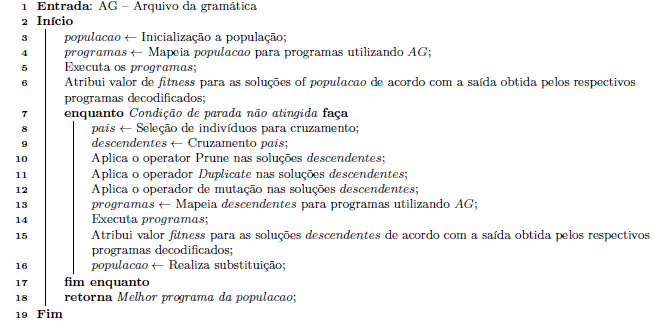
\includegraphics[scale=.6]{figuras/PseudocodigoEG.png}
					\caption{Pseudocódigo da evolução gramatical.}
					\label{fig:pseudocodigoEG}
				\end{figure}
				


}

